\documentclass[12pt]{article}
\usepackage{amsmath}
\usepackage{amssymb}
\usepackage{tikz}
\usetikzlibrary{arrows,positioning}

\begin{document}

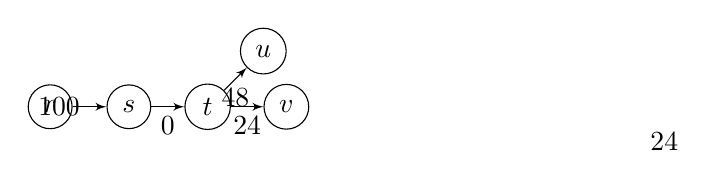
\begin{tikzpicture}[node distance=1cm]
    \tikzset{vertex/.style = {shape=circle,draw,minimum size=1.5em}}
    \tikzset{edge/.style = {->,> = latex'}}
    
    \node[vertex] (r) at (-3,0) {$r$};
    \node[vertex] (s) at (-1,0) [right of=r] {$s$};
    \node[vertex] (t) at (1,0) [right of=s] {$t$};
    \node[vertex] (u) at (1,2) [above right of=t] {$u$};
    \node[vertex] (v) at (4,0) [right of=t] {$v$};
    
    \path[edge] (r) edge node [left] {100} (s);
    \path[edge] (s) edge node [below] {0} (t);
    \path[edge] (t) edge node [below] {48} (u) 
                 (t) edge node [below] {24} (v);

    % Add vertex v label if needed
    \node at (4.5, -0.2) [below right] {24};

\end{tikzpicture}

The tree \( G \), weight distribution \( w \), and vertex \( v \) from the proof of~\Cref{prop:counterexample}.

\end{document}